% %% %%%%%%%%%%%%%%%%%%%%%%%%%%%%%%%%%%%%%%%%%%%%%%%%%%%%%%%%%%
% intro-i2c.tex
%
% Author:  Mauricio Matamoros
% License: MIT
%
% %% %%%%%%%%%%%%%%%%%%%%%%%%%%%%%%%%%%%%%%%%%%%%%%%%%%%%%%%%%%
%!TEX root = ../practica.tex
%!TEX root = ../references.bib

% CHKTEX-FILE 1
% CHKTEX-FILE 13
% CHKTEX-FILE 46

\subsection{Bus \IIC}%
\label{seq:intro-i2c}
\begin{wrapfigure}{r}{0.3\columnwidth}
	\centering
	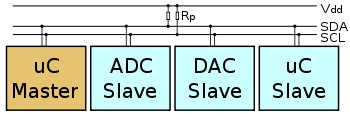
\includegraphics[width=0.3\columnwidth]{img/i2c-bus.png}
	\caption{Bus \IIC}%
	\label{fig:iic-bus}
\end{wrapfigure}
\IIC es un protocolo serial inventado por Phillips y diseñado para conectar dispositivos de baja velocidad mediante interfaces de dos hilos (\Cref{fig:iic-bus}).
El protocolo permite un número virtualmente ilimitado de dispositivos interconectados donde más de uno puede ser un dispositivo maestro.
El bus I2C es popular debido a su facilidad de uso y fácil configuración.
Sólo es necesario definir la velocidad máxima del bus, que está conformado por dos cables con resistencias pull-up~\Citep{IICWeb}.

\IIC utiliza solamente dos cables: SCL (reloj) y SDA (datos).
La transferencia de datos es serial y transmite paquetes de 8 bits con velocidades de hasta 5MHz.
Además, es requisito que cada dispositivo esclavo tenga una dirección de 7 bits que (el bit más significativo se utiliza para indicar si el paquete es una lectura o una escritura) debe ser única en el bus.
Los dispositivos maestros no necesitan dirección ya que estos generan la señal de reloj y coordinan a los dispositivos esclavos~\Citep{IICWeb}.
